\documentclass[11pt]{article}
\usepackage[margin=1in]{geometry}
\usepackage{amsmath}
\usepackage{amssymb}
\usepackage{tikz}
\usetikzlibrary{arrows.meta, positioning, shapes.geometric}

\title{Spike Simulator Adapter (Phase-2)}
\author{SIT Engine Phase-2}
\date{\today}

\begin{document}
\maketitle

\section{Purpose}
This note explains how \texttt{Phase-2/adapters/spike\_adapter.py} maps Spike commit-log output into Phase-2 normalized intervals:
\begin{itemize}
  \item \texttt{state\_intervals.csv}: \texttt{start\_us,end\_us,core,state}
  \item \texttt{residency\_intervals.csv}: \texttt{start\_us,end\_us,core,resident}
\end{itemize}

\section{Time and Core Mapping}
For each core, instructions are indexed in commit order. Timestamp is:
\[
t_{c,k} = k \cdot \Delta t_{inst}
\]
where \(k\) is per-core instruction count and \(\Delta t_{inst}=\texttt{inst\_us}\).

Core ID is extracted from \texttt{core N} (or fallback \texttt{hart N}) patterns in the Spike log.

\section{Residency Detection}
\subsection*{Marker-driven (preferred)}
Instruction encodings:
\[
\texttt{RES\_ON} = 0x06500013,\quad \texttt{RES\_OFF} = 0x06600013
\]
open/close residency spans directly.

\subsection*{PC-threshold fallback}
Used only if markers are never seen on a core:
\[
resident(t)=
\begin{cases}
1 & pc(t)\ge pc_{th}\\
0 & \text{otherwise}
\end{cases}
\]
with \(pc_{th}=\texttt{resident\_pc\_ge}\).

\section{State Inference}
Within residency intervals only, classify each instruction event into:
\[
state(t)=
\begin{cases}
\text{idle} & \text{if idle-rule mnemonic match}\\
\text{stall} & \text{if stall-rule mnemonic match}\\
\text{active} & \text{otherwise}
\end{cases}
\]

Idle-rule examples: \texttt{nop}, \texttt{c.nop}, residency marker ops, branch-loop maintenance, \texttt{fence*}, \texttt{csrr*}.\\
Stall-rule examples: load/store classes, compressed memory ops, \texttt{lr/sc/amo}.

\section{Interval Construction}
State intervals are emitted on state transition boundaries and closed at residency exits or trace end. Gaps are filled as idle to preserve contiguous per-core timelines.

Residency intervals are emitted from marker spans (preferred) or fallback spans.

\section{Flowchart}
\begin{center}
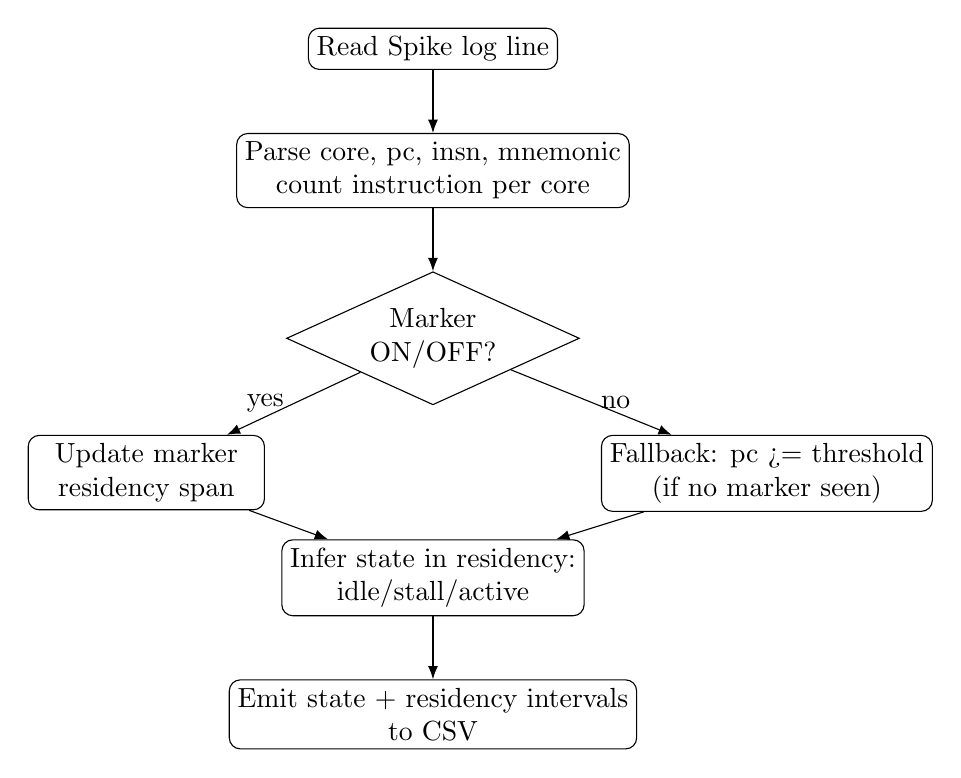
\begin{tikzpicture}[
  node distance=8mm and 12mm,
  box/.style={rectangle, draw, rounded corners, align=center, inner sep=3pt, minimum width=30mm},
  decision/.style={diamond, draw, aspect=2.2, align=center, inner sep=2pt},
  line/.style={-Latex}
]
\node[box] (start) {Read Spike log line};
\node[box, below=of start] (parse) {Parse core, pc, insn, mnemonic\\count instruction per core};
\node[decision, below=of parse] (marker) {Marker\\ON/OFF?};
\node[box, below left=of marker] (resm) {Update marker\\residency span};
\node[box, below right=of marker] (resf) {Fallback: pc >= threshold\\(if no marker seen)};
\node[box, below=17mm of marker] (state) {Infer state in residency:\\idle/stall/active};
\node[box, below=of state] (emit) {Emit state + residency intervals\\to CSV};

\draw[line] (start) -- (parse);
\draw[line] (parse) -- (marker);
\draw[line] (marker) -- node[left]{yes} (resm);
\draw[line] (marker) -- node[right]{no} (resf);
\draw[line] (resm) -- (state);
\draw[line] (resf) -- (state);
\draw[line] (state) -- (emit);
\end{tikzpicture}
\end{center}

\section{CLI}
\begin{verbatim}
python Phase-2/adapters/spike_adapter.py \
  --spike-trace <spike.trace> \
  --out-dir <run/inputs> \
  --inst-us 1.0 \
  --resident-pc-ge 0x80000000
\end{verbatim}

\end{document}

